\chapter{Aplicación: Sitio Web (Website Builder)}
\label{ch:sitio_web}

Odoo no solo es un sistema de gestión interno (backend), sino que incluye un potente constructor de páginas web (frontend). El módulo \textbf{Sitio Web} te permite diseñar la página pública de la agencia, crear blogs, páginas de destino (landing pages) y gestionar la tienda en línea (eCommerce) donde los pasajeros pueden comprar tours directamente.

En esta sección aprenderás a navegar por la interfaz de diseño (Website Builder) y realizar modificaciones directamente en la página con el enfoque "Lo que ves es lo que obtienes" (WYSIWYG).

\section{Modo de Edición (Website Builder)}

Para empezar a modificar cualquier página, el primer paso es ingresar a la aplicación \textbf{Sitio Web} desde el menú principal. Al hacerlo, el sistema te redirigirá a la vista frontal de la página de inicio, pero con una barra oscura en la parte superior exclusiva para administradores.

\subsection{1. Activar el Editor (Update)}

\begin{figure}[H]
    \centering
    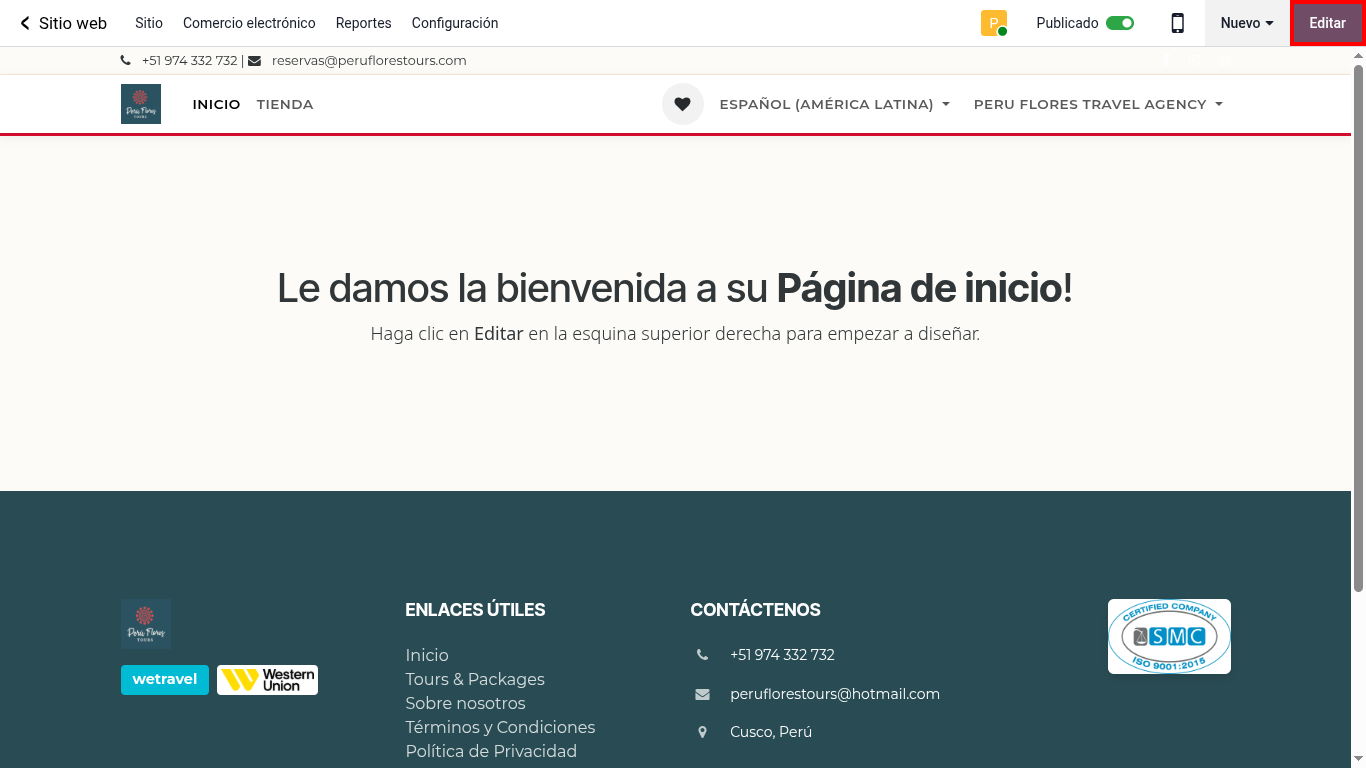
\includegraphics[width=0.9\textwidth]{assets/web_01_boton_editar.png}
    \caption{Botón "Editar" (resaltado en rojo) en la esquina superior derecha.}
\end{figure}

Para cambiar cualquier texto, imagen o estructura de la página que estás viendo, simplemente haz clic en el botón \textbf{``Editar''}. Odoo transformará la página estática en un lienzo interactivo.

\subsection{2. El Panel de Bloques (Estructuras y Diseño)}

\begin{figure}[H]
    \centering
    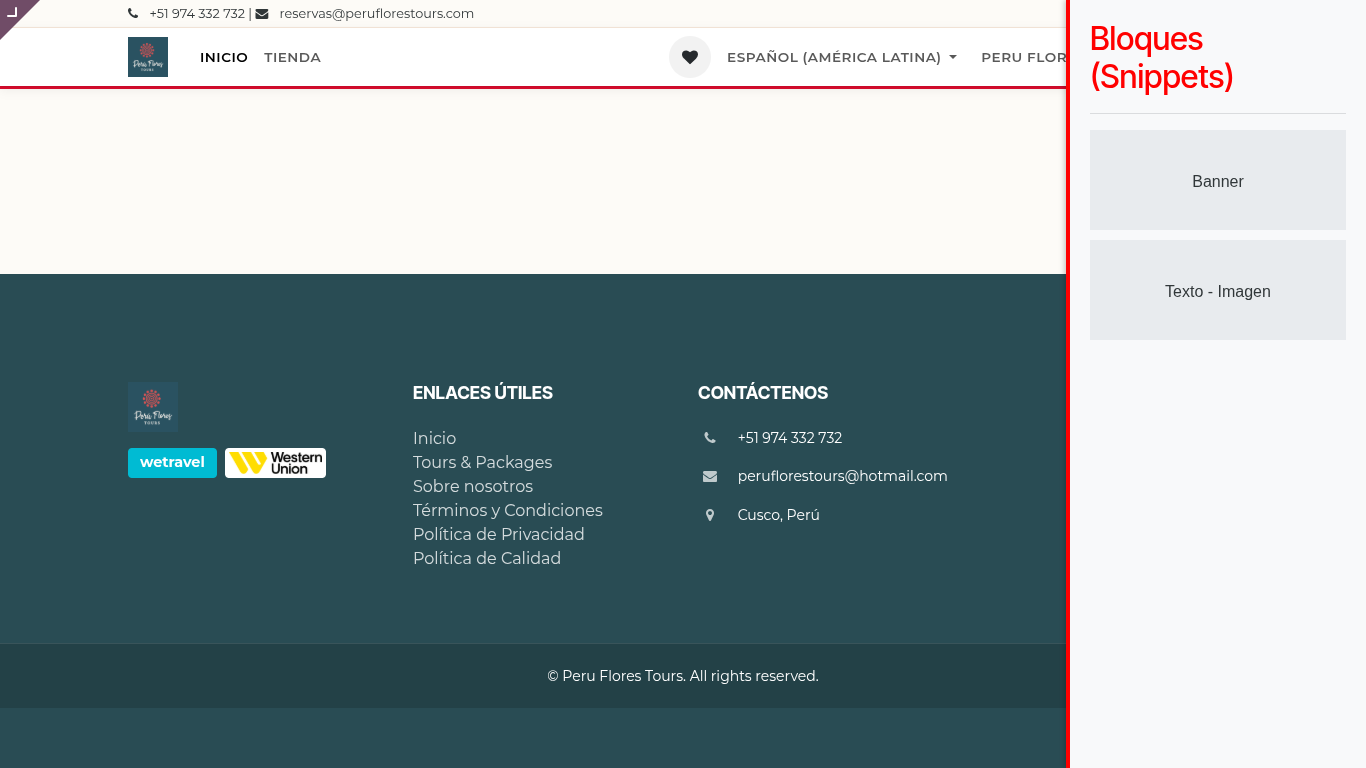
\includegraphics[width=0.9\textwidth]{assets/web_02_panel_bloques.png}
    \caption{El Panel de Snippets/Bloques (resaltado en rojo) a la derecha de la pantalla.}
\end{figure}

Al entrar en modo edición, aparecerá el panel lateral de Odoo. Este panel está dividido en dos partes:
\begin{itemize}
    \item \textbf{Bloques (Snippets):} Estructuras pre-diseñadas (Ej: Carrusel de imágenes, Banner, Texto + Foto, Tres columnas, etc.) que puedes simplemente arrastrar y soltar en la página.
    \item \textbf{Personalizar:} Si haces clic sobre cualquier elemento de la página (un texto, un botón, una imagen), el panel lateral cambiará para mostrarte las opciones de diseño de ese elemento (color, tamaño, bordes, enlaces).
\end{itemize}

\subsection{3. Guardar los Cambios}

\begin{figure}[H]
    \centering
    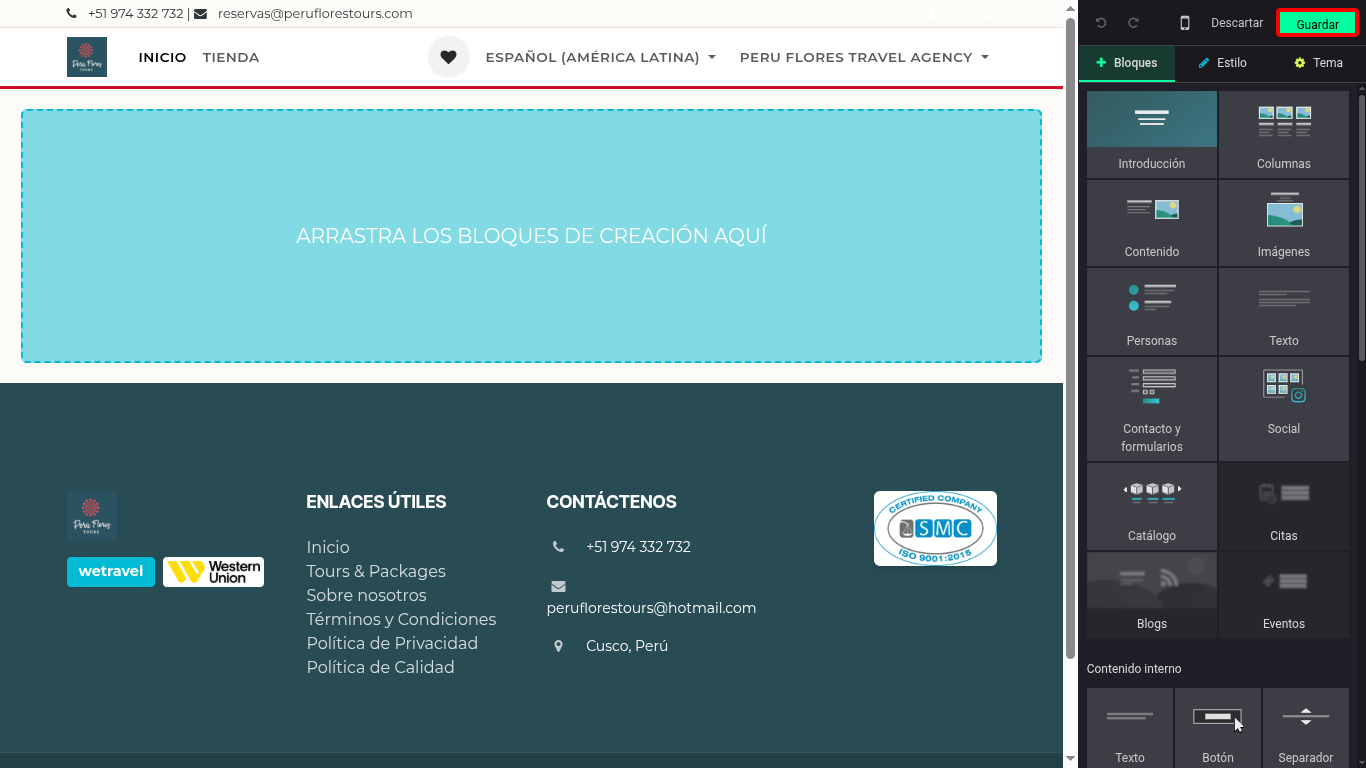
\includegraphics[width=0.9\textwidth]{assets/web_03_boton_guardar.png}
    \caption{Botón "Guardar" (resaltado en rojo) para aplicar los cambios públicamente.}
\end{figure}

Una vez que arrastraste tus bloques, editaste los textos haciendo clic directamente sobre ellos y cambiaste las imágenes, \textbf{debes hacer clic en Guardar} en la esquina superior derecha. Si te equivocaste y quieres deshacer todo, haz clic en \textbf{Descartar}.

\section{Crear y Gestionar Contenido}

Además de editar las páginas existentes, puedes crear nuevas secciones desde cero (Create).

\subsection{4. Crear Nuevas Páginas (Create)}

\begin{figure}[H]
    \centering
    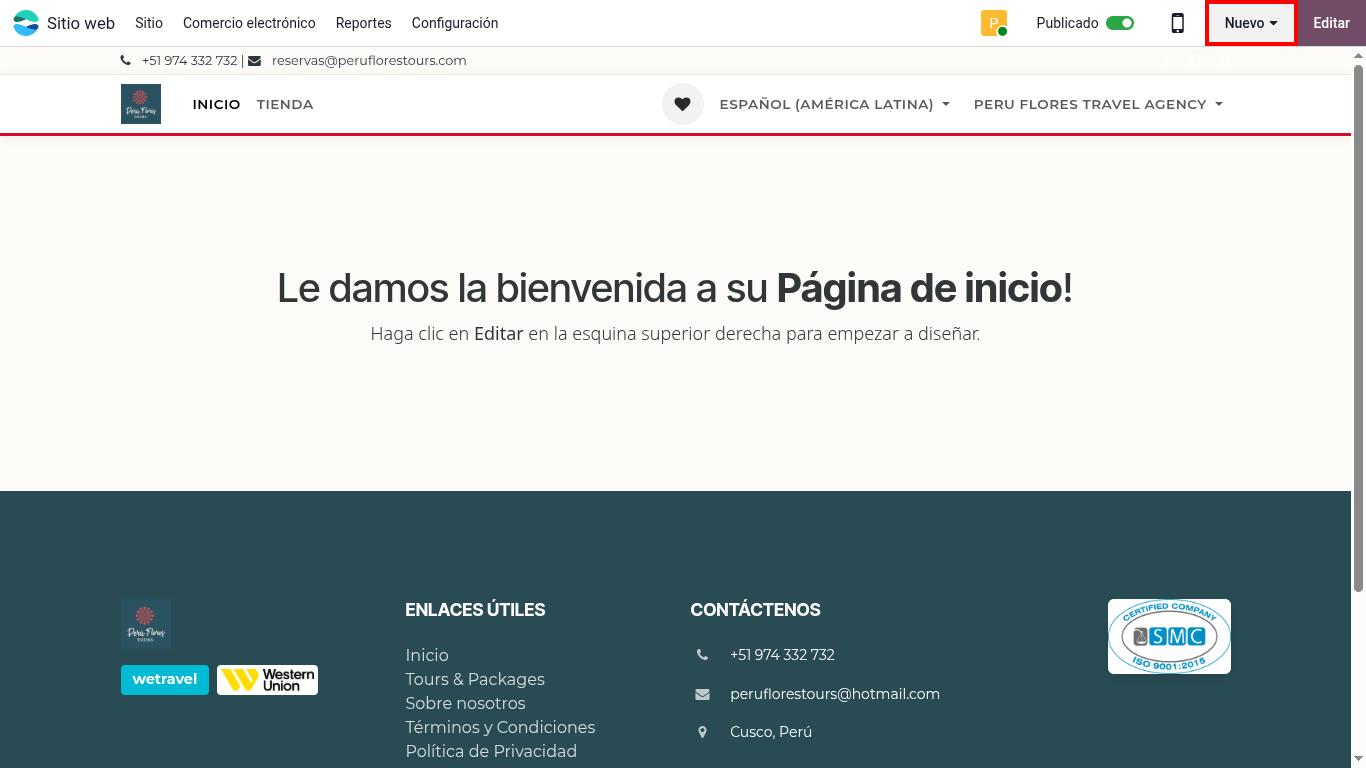
\includegraphics[width=0.9\textwidth]{assets/web_04_boton_nuevo.png}
    \caption{El botón "Nuevo" (resaltado en rojo) en la barra superior.}
\end{figure}

Si la agencia lanza una nueva campaña o necesita una página específica para un grupo escolar, haz clic en el botón \textbf{+ Nuevo}. 

\begin{figure}[H]
    \centering
    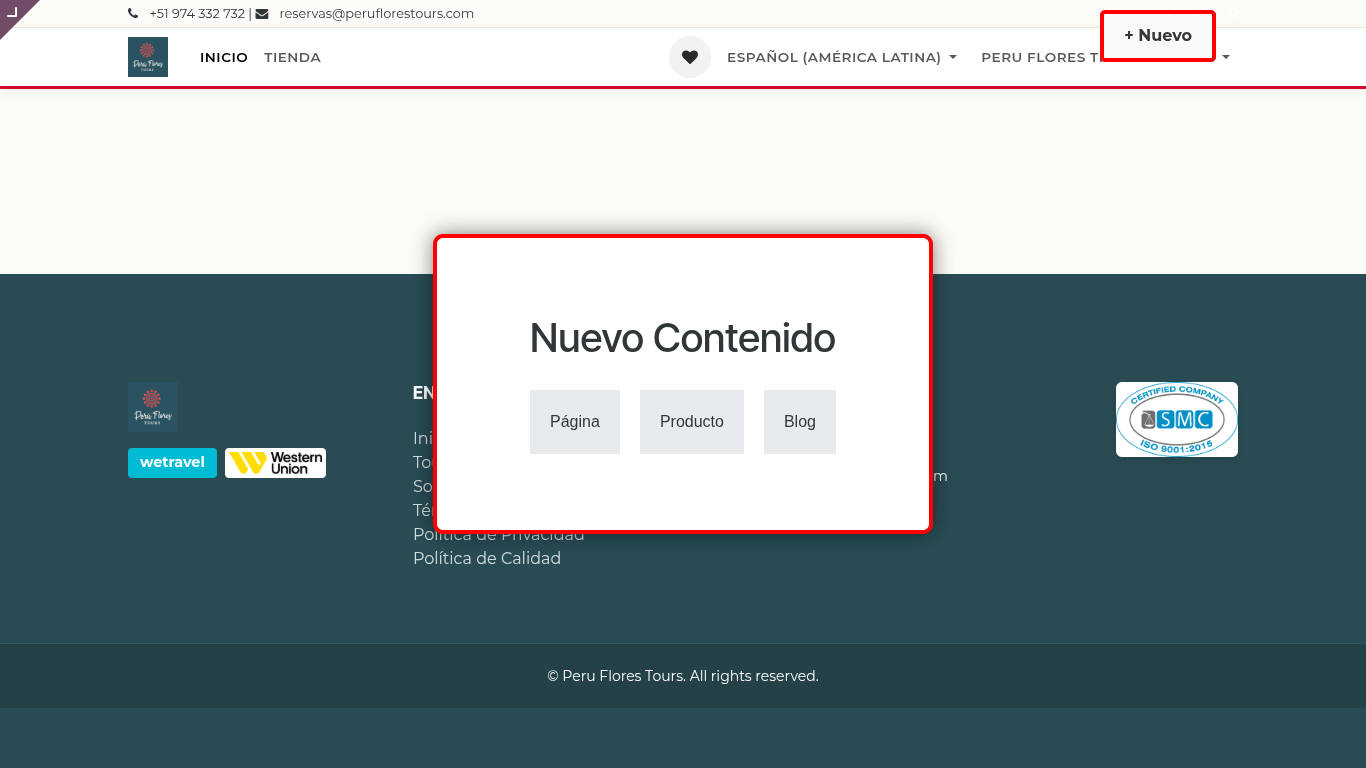
\includegraphics[width=0.9\textwidth]{assets/web_05_modal_nuevo.png}
    \caption{Menú emergente (modal) con las opciones de contenido nuevo.}
\end{figure}

Odoo te preguntará qué tipo de contenido deseas crear:
\begin{itemize}
    \item \textbf{Página:} Una nueva página web en blanco.
    \item \textbf{Entrada de Blog:} Un artículo de noticias o recomendaciones turísticas.
    \item \textbf{Producto:} Un nuevo tour para la tienda online (esto es el equivalente a crearlo desde el catálogo backend, pero aquí puedes ver cómo lucirá públicamente).
\end{itemize}

\subsection{5. Editar el Menú Principal (Navegación)}

\begin{figure}[H]
    \centering
    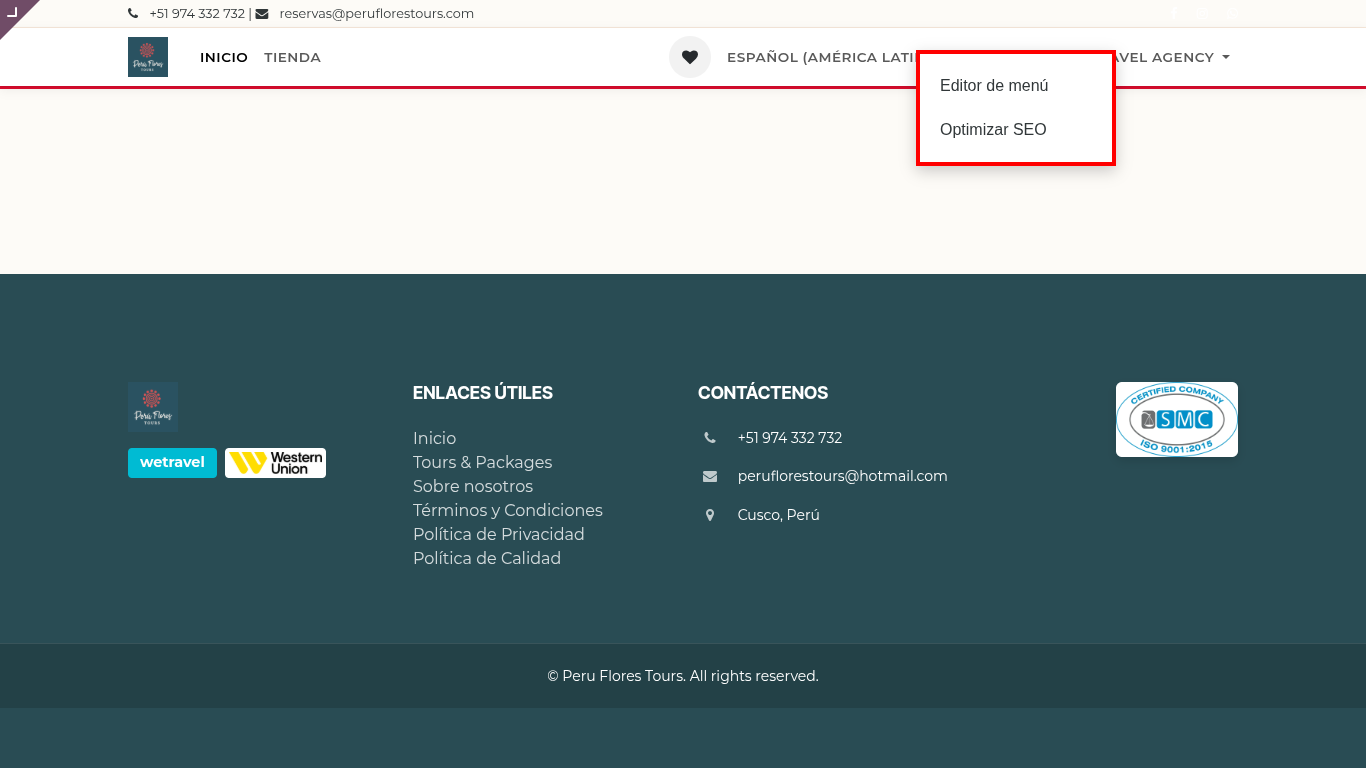
\includegraphics[width=0.9\textwidth]{assets/web_06_editor_menu.png}
    \caption{El menú Sitio $>$ Editor de Menú resaltado en rojo.}
\end{figure}

Si creaste una nueva página y quieres que aparezca en la barra de navegación superior (Ej: Inicio, Tours, Sobre Nosotros, Contacto), debes ir a \textbf{Sitio > Editor de menú}. Allí podrás añadir nuevos enlaces, organizar el orden arrastrándolos, y crear submenús desplegables.

\section{Regla de Oro del eCommerce}

Aunque la tienda online (eCommerce) está dentro del Sitio Web, recuerda que todos los tours que vendas por internet nacen del \textbf{Catálogo de Productos}. Si necesitas cambiar un precio o la categoría del tour, es mucho más rápido hacerlo desde el módulo de Ventas (o Productos) que buscarlo en el sitio web. El sitio web simplemente "refleja" y "publica" lo que configuras en tu backend.
